% The arithmetic of the kernel: how RVD's predicates get exact signs.
%
% A companion to ../predicates/side_predicates.tex (what the predicates
% compute), to ../../design_document/DESIGN.tex (section 6), and to the
% headers of code/src/kernel/. Build with
%
%   latexmk -pdf arithmetic.tex        or        pdflatex arithmetic.tex (twice)
\documentclass[11pt,a4paper]{article}

\usepackage[T1]{fontenc}
\usepackage[utf8]{inputenc}
\usepackage{lmodern}
\usepackage[british]{babel}
\usepackage[a4paper,margin=2.5cm]{geometry}
\usepackage{microtype}
\usepackage{amsmath,amssymb,amsthm,mathtools}
\usepackage{array,booktabs,tabularx}
\usepackage[shortlabels]{enumitem}
\usepackage{xcolor}
\usepackage{tikz}
\usetikzlibrary{arrows.meta,calc,positioning,shapes.geometric}
\usepackage{caption}
\usepackage[colorlinks,linkcolor=blue!50!black,urlcolor=blue!50!black]{hyperref}

\newcommand{\code}[1]{\texttt{#1}}
\newcommand{\R}{\mathbb{R}}
\newcommand{\norm}[1]{\lVert #1\rVert}
\newcommand{\sgn}{\operatorname{sign}}
\newcommand{\fl}{\operatorname{fl}}
\newcommand{\ulp}{\operatorname{ulp}}
\newcommand{\secref}[1]{\S\ref{#1}}
\newcolumntype{L}{>{\raggedright\arraybackslash}X}
\renewcommand{\arraystretch}{1.2}
\setlist{itemsep=2pt,topsep=4pt}

\newtheorem{lemma}{Lemma}
\newtheorem{theorem}{Theorem}
\theoremstyle{definition}
\newtheorem{definition}{Definition}
\theoremstyle{remark}
\newtheorem*{remark}{Remark}
\newtheorem*{example}{Example}

\newcommand{\keybox}[1]{%
  \begin{center}\fbox{\begin{minipage}{0.94\linewidth}\smallskip #1\smallskip\end{minipage}}\end{center}}

\title{\textbf{The arithmetic of the kernel}\\[0.4em]
  \large How RVD's predicates get exact signs: error-free transformations, expansions,\\
  the filter, and Simulation of Simplicity}
\author{}
\date{5 October 2026}

\begin{document}
\maketitle

\keybox{\small
  \textbf{What this is.} A reference to come back to when the arithmetic of
  \code{code/src/kernel/} stops making sense. It explains, from the bottom up, why a
  predicate cannot simply be evaluated in \code{double}, and how each layer of the kernel
  fixes one part of that: the error-free transformations of \code{eft.h}, the expansions of
  \code{expansion.h} and \code{dynamic\_expansion.h}, the filter of \code{bounded.h}, and the
  symbolic perturbation that step~7 adds on top. Each section gives the theory, says where it
  lives in the code, and gives a worked example small enough to check by hand. The companion
  document \code{documents/predicates/side\_predicates.tex} derives the formulas the
  predicates evaluate; this one is about \emph{how} they are evaluated.

  \smallskip
  \textbf{State, 5 October 2026.} Everything up to \code{side4} is written and tested.
  Symbolic perturbation (\secref{sec:sos}) is designed and its tests are written and
  validated; \code{side1\_sos} is written and passes, \code{side2\_sos} to \code{side4\_sos} are
  next. The measured numbers are in \secref{sec:measured}, with how to reproduce them.}

\tableofcontents

% ======================================================================================
\section{The problem, and the plan}\label{sec:problem}

\subsection{A predicate is the sign of a polynomial}

Every decision the clipper takes is a \emph{predicate}: a question with a discrete answer,
such as ``is this vertex on seed $i$'s side of the bisector of $i$ and $m$?''. Each one is the
sign of a polynomial in the input numbers: \code{orient2d} is a $2\times2$ determinant of
coordinate differences (degree 2), \code{orient3d} a $3\times3$ one (degree 3), and the side
predicates are ratios of determinants of degree up to 6 over 4. The value itself is never
needed, only whether it is negative, zero or positive.

\subsection{Why doubles get the sign wrong}

A \code{double} holds 53 significant bits, and each operation rounds its exact result to the
nearest double. A polynomial of degree 6 in 53-bit inputs can need a few hundred bits to be
written exactly, and near a degeneracy -- a point almost on a line, a vertex almost on a
bisector -- the exact value is tiny while the rounding errors of the terms that nearly cancel
are not. Then the computed value can have the wrong sign, or be zero when the true value is
not, or the other way round.

This is not a rare corner case in a Voronoi code. Two cells look at the same vertex, each
through its own computation, and if their roundings disagree, one cell thinks a facet exists
and the other does not: the diagram has a crack. On a regular lattice of seeds, every vertex is
a degeneracy. Measured on the side predicates' test inputs (\secref{sec:measured}): on ties
moved by one ulp, constructing the vertex in doubles and comparing distances got 65\% to 76\% of
the signs wrong.

\subsection{Three layers}

The kernel computes each sign in up to three steps (figure~\ref{fig:pipeline}), following
DESIGN.tex, section 6.3:

\begin{enumerate}
  \item \textbf{The filter} (\secref{sec:filter}). Evaluate the polynomial in doubles, and
    alongside it a certified bound on the rounding error. If the value is farther from zero
    than the bound, its sign is proven. On random inputs this decided 98\% to 100\% of calls, at
    3 to 13 times the cost of a plain double evaluation (\secref{sec:measured}).
  \item \textbf{The exact path} (\secref{sec:eft} to \secref{sec:dynamic}). Otherwise evaluate
    the same polynomial exactly, as an \emph{expansion}: an unevaluated sum of doubles built
    from error-free operations. Its sign is the true sign, zero included.
  \item \textbf{Symbolic perturbation} (\secref{sec:sos}). If the exact value is zero, answer
    the question for an imaginary, infinitesimally perturbed input instead, the same one for
    every predicate, so that ties are broken consistently and no predicate ever answers 0.
\end{enumerate}

\begin{figure}[ht]
\centering
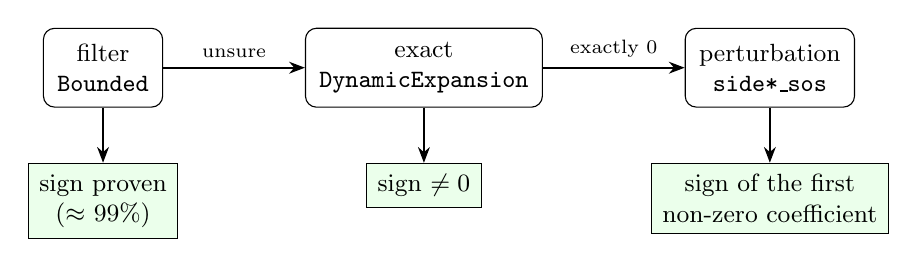
\begin{tikzpicture}[
    node distance=7mm and 18mm,
    box/.style={draw, rounded corners, align=center, inner sep=5pt, font=\small,
                minimum height=10mm},
    ans/.style={draw, align=center, inner sep=4pt, font=\small, fill=green!8},
    arr/.style={-{Stealth[length=2mm]}, thick},
    lab/.style={font=\scriptsize, midway}]
  \node[box] (filter) {filter\\ \code{Bounded}};
  \node[box, right=of filter] (exact) {exact\\ \code{DynamicExpansion}};
  \node[box, right=of exact] (sos) {perturbation\\ \code{side*\_sos}};
  \node[ans, below=of filter] (a1) {sign proven\\ ($\approx$ 99\%)};
  \node[ans, below=of exact] (a2) {sign $\neq 0$};
  \node[ans, below=of sos] (a3) {sign of the first\\ non-zero coefficient};
  \draw[arr] (filter) -- node[lab, above] {unsure} (exact);
  \draw[arr] (exact) -- node[lab, above] {exactly 0} (sos);
  \draw[arr] (filter) -- (a1);
  \draw[arr] (exact) -- (a2);
  \draw[arr] (sos) -- (a3);
\end{tikzpicture}
\caption{How one predicate call is decided. Each step runs only if the one before could not
decide. The counters of \code{predicate\_counts.h} record which step did.}
\label{fig:pipeline}
\end{figure}

The rest of this document goes bottom-up: floating point (\secref{sec:fp}), the error-free
transformations (\secref{sec:eft}), expansions (\secref{sec:expansions}), the two containers
(\secref{sec:dynamic}), the filter (\secref{sec:filter}), how a predicate combines them
(\secref{sec:together}), and the perturbation (\secref{sec:sos}).

% ======================================================================================
\section{Floating point, in one page}\label{sec:fp}

\subsection{What a double is}



So binary64 number has the components: sign, significand, and exponent. In binary notation 
$x=(-1)^s (1.f_1f_2\dots f_{52})_2 2^{E-1023}$. So sign takes 1 bit, exponent takes 11 bits, and the significand 
takes then 52 bits. But since every normalized binary number, like shown in the binary notation, has the first bit 1, 
we can ignore that and "win" one more bit for the significand. This win in precision is called 
\textbf{implicit 1} or \textbf{hidden bit}. This does not mean 53 bits are stored but just 
assumed in the normal case that the leading bit is 1 and it is the most 
significant bit.
The exponent is stored biased. Meaning $e = E - 1023$, so that we do not have to deal 
with signed bit ordering, it is just unsigned bit ordering for 11 bits. And like this we also can 
reserve all-zero or all-one bit patterns for special values.
On the computer the bits are stored in the order: sign(1 bit), exponent (11 bits), significand (52 bits).


Two quantities appear everywhere:
\begin{itemize}
  \item $\ulp(x)$, the \emph{unit in the last place}: the gap between $x$ and the next double
    away from zero. For $1 \le |x| < 2$ it is $2^{-52}$.
  \item $u = 2^{-53}$, the \emph{unit roundoff}: half an ulp of 1. In \code{bounded.h} it is
    \code{kU}.
\end{itemize}

For a \textbf{normal} number we have $E \in 1, \dots, 2046$. The exponent values $E=0$ (zero or subnormal) and 
$E = 2047$ ($\infty$ or $NaN$) are deliberately reserved. 

When $E=0$, the hidden 1 is removed and the formula becomes
$$
x = (-1)^s (0.f)_2 2^{-1022}
$$
these are subnormal numbers. Why $-1022$? With the smallest normal $E=1$, we get 
the smallest normal exponent $e=-1022$. So the smallest normal positive number is 
$$
1.0\dots 0_2 \times 2^{-1022} = 2^{-1022}
$$
Now we also want to represent numbers below this, otherwise we jump directly to $0$ after this 
smallest normal number. \textbf{Subnormals} fill that region. With this, the smallest positive binary64 number is 
$2^{-1074}$.

Another special case is when $E=0$ and all significand bits 0. Then $x=(-1)^s 0.0\dots0 2^0$. This gives 
two floating point zeros, one with positive sign and the other with a negative sign.

Another special case is when $E = 2^{12} - 1$. Here the significand bits determine if we get infinity or $NaN$. 
If significand bits are zero we get infinity (again with two signs). When significand bits are not zero then 
we get "not a number".

\subsection{Rounding}

Every operation $\circ \in \{+,-,\times\}$ returns $\fl(a \circ b)$, the exact result rounded
to the nearest double; a tie, exactly halfway between two doubles, goes to the one whose last
bit is 0 (\emph{round to nearest, ties to even}, the IEEE~754 default). In the normal range,
\[
  \fl(x) = x(1 + \delta), \qquad |\delta| \le u .
\]
That one inequality is all the filter (\secref{sec:filter}) needs. The exact path needs three
sharper facts (listed in \code{eft.h} as F1--F3):

\begin{description}
  \item[F1] The rounding error of a sum is a double: $a + b - \fl(a+b)$ is representable,
    and at most $\tfrac12\ulp(\fl(a+b))$.
  \item[F2] \emph{Sterbenz's lemma}: if $b/2 \le a \le 2b$, then $a - b$ is computed exactly.
  \item[F3] The rounding error of a product is a double, provided it does not underflow: the
    exact product of two 53-bit significands has at most 106 bits, so $ab - \fl(ab)$ has at
    most 53.
\end{description}

\subsection{What the code must not let the compiler do}

These facts hold for the arithmetic they were proved for, so the build protects them:
\begin{itemize}
  \item \textbf{No} \code{-ffast-math}: it lets the compiler use real-number algebra, under
    which the error terms below are identically zero and get deleted.
  \item \code{-ffp-contract=off}, for every target: it stops the compiler fusing $a\times b + c$
    into one \code{fma}, which rounds once instead of twice and breaks the proofs. An explicit
    \code{std::fma}, as in \code{two\_product}, is still honoured.
  \item No extended precision: x86-64 and ARM compute doubles in 64-bit registers, so the old
    x87 ``double rounding'' problem does not arise.
\end{itemize}

\subsection{The range}

The guarantees fail near the ends of the range, and what fails is the \emph{error-free
transformation}, not just the rounded operation:
\begin{itemize}
  \item \code{two\_sum} and \code{fast\_two\_sum} are exact unless the sum overflows. With gradual
    underflow the rounding error of a sum is always representable, even among subnormals.
  \item \code{two\_product} is exact when the residual $ab - \fl(ab)$ is exactly representable.
    That can fail near underflow: a residual below the subnormal grid is lost. A simple
    \emph{sufficient} condition, the one the code relies on, is $|ab| \ge 2^{-969}$
    ($= 2^{-1022+53}$) or $ab = 0$.
\end{itemize}
The condition is on \emph{every intermediate product}, not on the inputs: two normal inputs near
$2^{-600}$ already have a product that underflows. A predicate of degree 6 multiplies six
inputs, so inputs must be zero or of moderate size: the side-predicate tests keep exponents in
$[-20, 20]$, and a first draft that nudged a zero coordinate to the smallest subnormal
($2^{-1074}$, whose square underflows to 0) broke exactness at once. Checking the range belongs
where a domain or a seed set is built.

% ======================================================================================
\section{Error-free transformations}\label{sec:eft}

An \emph{error-free transformation} (EFT) turns one rounded operation into two doubles whose
\emph{sum is the exact result}:
\[
  \code{two\_sum}(a,b) = \{h, \ell\}:\quad h = \fl(a+b),\quad h + \ell = a + b \text{ exactly};
\]
and the same for products. The second double $\ell$ is the rounding error, which F1 and F3
say is itself a double; the algorithms compute it exactly, using nothing but more rounded
operations. The results of the sum and product EFTs (\code{two\_sum}, \code{fast\_two\_sum},
\code{two\_product}, \code{two\_product\_dekker}) also satisfy $|\ell| \le \tfrac12\ulp(h)$: the
two parts cover disjoint ranges of bits, and $h + \ell$ rounds back to $h$. \code{split} is
different (\secref{ssec:split}): its parts do not overlap either, but its low part is only bounded
by half a unit of the high part's 26th bit, which can be about $2^{27}$ times $\tfrac12\ulp(h)$.
All of \code{kernel/eft.h} is five such functions, and everything exact in RVD is built from
them.

\subsection{\texorpdfstring{\code{fast\_two\_sum}}{fast\_two\_sum}: three operations, one precondition}

Shewchuk's Theorem 6 (after Dekker): if $|a| \ge |b|$, then
\[
  h = \fl(a+b),\qquad b_v = h - a,\qquad \ell = b - b_v
\]
gives $h + \ell = a + b$ exactly. The idea: because $b$ is the smaller term, $h - a$ is
computed exactly, so $b_v$ is \emph{exactly} the part of $b$ that made it into $h$; then
$b - b_v$, the part that did not, is the rounding error, a double by F1, so that subtraction is
exact too. Without $|a| \ge |b|$ the first subtraction can round and $\ell$ is wrong, which is
why the code asserts the precondition, and why the tests compile with asserts on.

\subsection{\texorpdfstring{\code{two\_sum}}{two\_sum}: six operations, no precondition}

Shewchuk's Theorem 7 (after Knuth) removes the precondition by recovering both operands:
\begin{align*}
  h &= \fl(a+b), & b_v &= h - a, & a_v &= h - b_v,\\
  b_r &= b - b_v, & a_r &= a - a_v, & \ell &= a_r + b_r .
\end{align*}
When $|b| > |a|$ the recovered $b_v$ and $a_v$ may themselves be rounded, but the errors made in
recovering them cancel exactly in $a_r + b_r$.

\begin{example}
$\code{two\_sum}(2^{53}, 1)$: the exact sum $2^{53}+1$ lies halfway between the doubles $2^{53}$
and $2^{53}+2$; the tie goes to the even one, so $h = 2^{53}$, and $\ell = 1$. The pair
$\{2^{53}, 1\}$ holds the exact sum, which no single double can.
\end{example}

\subsection{\texorpdfstring{\code{two\_product}}{two\_product}: two operations, with fma}

$h = \fl(ab)$ and $\ell = \code{fma}(a, b, -h)$. The fma computes $ab - h$ with a single rounding;
that exact value is a double by F3, so rounding it changes nothing, and $\ell$ is the exact
error. It is fast wherever the CPU has an fma instruction: most x86-64 processors since Intel's
Haswell and AMD's Piledriver, and every 64-bit ARM. Not all: Pentium- and Celeron-branded parts of
those generations, and several Atom cores, have none, and then \code{std::fma} is emulated in
software, slowly.

\subsection{\texorpdfstring{\code{split}}{split} and \texorpdfstring{\code{two\_product\_dekker}}{two\_product\_dekker}: the same without fma}\label{ssec:split}

Shewchuk's Theorems 17 and 18 (Dekker, after Veltkamp). \code{split} cuts $a$ into two halves of
at most 26 significant bits each, using the constant $2^{27}+1$; two such halves multiply to at
most 52 bits, which fits a double exactly. So $ab$ is the exact sum of four exact products of
halves, and peeling them off $h$ largest first, each subtraction exact, leaves the error. Kept
because it is what to use where fma is emulated in software, and tested to give the same
$h$ and $\ell$ as \code{two\_product} (compared with \code{==}, so a $+0$ and a $-0$ count as
equal).

% ======================================================================================
\section{Expansions}\label{sec:expansions}

\subsection{Definition}

An \emph{expansion} is a finite list of doubles whose \emph{exact} sum is the number it
represents:
\[
  x = c_0 + c_1 + \cdots + c_{n-1} \qquad \text{in the real numbers.}
\]
Its components are kept in a strict normal form, the \textbf{invariant} that every operation
assumes of its inputs and must restore in its result:
\begin{itemize}
  \item \textbf{nonzero} -- zero is the empty list, never a component;
  \item \textbf{nonoverlapping} -- see below;
  \item \textbf{increasing magnitude} -- smallest first, $|c_0| < |c_1| < \cdots < |c_{n-1}|$.
\end{itemize}
In both containers \code{append()} is the only way a component gets in. It drops zeros,
asserts that each new component is larger in magnitude than the last, and in \code{Expansion<N>}
asserts that there is room. It does \emph{not} check nonoverlap: that is each operation's theorem,
and the tests check it against exact rationals after every operation.

\subsection{Nonoverlapping, nonadjacent, strongly nonoverlapping}

Write a double's binary magnitude as a string of bits; say it \emph{covers} the positions from
its lowest set bit to its highest. Shewchuk's definitions (nonoverlapping, adjacent and
nonadjacent in his section 2.1; strongly nonoverlapping in section 2.4, next to Theorem 13):

\begin{definition}
Two doubles $x$, $y$ are \textbf{nonoverlapping} if the lowest set bit of one is above the
highest set bit of the other: they cover disjoint ranges of positions. They are
\textbf{adjacent} if they overlap, or if $x$ overlaps $2y$, or $2x$ overlaps $y$: they touch,
one's highest bit sitting right below the other's lowest. An expansion is
\begin{itemize}
  \item \emph{nonoverlapping} if no two components overlap;
  \item \emph{nonadjacent} if no two components are adjacent;
  \item \emph{strongly nonoverlapping} if it is nonoverlapping, no component is adjacent to two
    others, and any two adjacent components are both powers of two.
\end{itemize}
\end{definition}

\begin{figure}[ht]
\centering
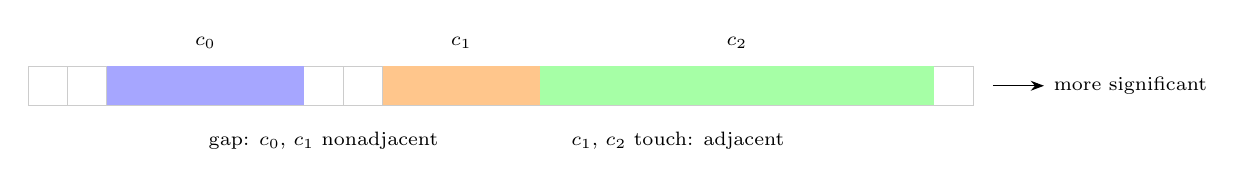
\begin{tikzpicture}[x=5mm, y=5mm, every node/.style={font=\scriptsize}]
  \foreach \i in {0,...,23} { \draw[gray!40] (\i,0) rectangle (\i+1,1); }
  \foreach \i in {2,...,6}   { \fill[blue!35]   (\i,0) rectangle (\i+1,1); }
  \foreach \i in {9,...,12}  { \fill[orange!45] (\i,0) rectangle (\i+1,1); }
  \foreach \i in {13,...,22} { \fill[green!35]  (\i,0) rectangle (\i+1,1); }
  \node at (4.5,1.6) {$c_0$};
  \node at (11,1.6) {$c_1$};
  \node at (18,1.6) {$c_2$};
  \draw[-{Stealth}] (24.5,0.5) -- (25.8,0.5) node[right] {more significant};
  \node[align=center] at (7.5,-0.9) {gap: $c_0$, $c_1$ nonadjacent};
  \node[align=center] at (16.5,-0.9) {$c_1$, $c_2$ touch: adjacent};
\end{tikzpicture}
\caption{The bit ranges of a nonoverlapping expansion of three components, least significant
on the left. $c_1$ and $c_2$ touch, so the expansion is nonoverlapping but not nonadjacent; and
since they are not powers of two, not strongly nonoverlapping either.}
\label{fig:bits}
\end{figure}

\subsection{What the invariant buys}

\begin{lemma}[the sign is the sign of the largest component]\label{lem:sign}
In a nonoverlapping expansion, $|c_0 + \cdots + c_{n-2}| < |c_{n-1}|$.
\end{lemma}
\begin{proof}[Why]
All the smaller components lie in bit positions below the lowest set bit of $c_{n-1}$, and
in disjoint ranges, so their sum is less in magnitude than that lowest bit, which is at most
$|c_{n-1}|$.
\end{proof}

So a predicate's answer is one comparison: the sign of the last component, or 0 for the empty
expansion. This is \code{sign()}. But the largest component is \emph{not} a good approximation of
the value: $[1023.9,\ 1024]$ is nonoverlapping (all of $1023.9$ lies below $1024$'s single bit)
and is worth about twice its largest component. To read a value, add the components smallest
first: \code{approximate()}. A \emph{compressed} expansion (\secref{ssec:compress}) does have its
largest component within an ulp of the value.

\subsection{The operations}

Each operation is exact: it returns the exact sum, product or negation of its operands, as
another expansion. Theorem numbers are Shewchuk's (1997).

\begin{description}
  \item[\code{grow}$(e, b)$] $e + b$ for a double $b$ (Grow-Expansion, Theorem 10). Carry $b$ up
    through the components with \code{two\_sum}; each step's error is final, because everything
    still to come is larger and does not overlap it; the last carry is the largest component.
  \item[\code{sum}$(a, b)$] grow $a$ by each component of $b$ (Expansion-Sum, Theorem 12).
    $O(mn)$; kept as a reference for the faster ones.
  \item[\code{fast\_sum}$(a, b)$] merge $a$ and $b$ into one list by magnitude (as in merge
    sort), then one carry pass: \code{fast\_two\_sum} for the first two, \code{two\_sum} after
    (Fast-Expansion-Sum, Theorem 13). $O(m+n)$. Requires \emph{strongly} nonoverlapping inputs,
    and its promise to return one is false (\secref{ssec:thm13}); it is no longer used by the
    operators.
  \item[\code{linear\_sum}$(a, b)$] the same merge, with a carry kept as \emph{two} doubles, $Q$
    and $q$ (Linear-Expansion-Sum, Theorem 24, Shewchuk's appendix): each new $g_k$ first absorbs
    $q$ with a \code{fast\_two\_sum}, whose low part is final, and the rest goes into $Q$ with a
    \code{two\_sum}. Nonoverlapping inputs give a nonoverlapping result, under any tie rule.
    About half again \code{fast\_sum}'s work. \textbf{This is the sum the operators use.}
  \item[\code{scale}$(e, b)$] $e\cdot b$ for a double $b$ (Scale-Expansion, Theorem 19). Each
    component's \code{two\_product} is folded into the carry with a \code{two\_sum} and a
    \code{fast\_two\_sum}: two final components per input component. Nonoverlapping in,
    nonoverlapping out; nonadjacent in, nonadjacent out.
  \item[\code{product}$(a, b)$] $\sum_j \code{scale}(a, b_j)$, accumulated with
    \code{linear\_sum}. Every step is a theorem.
  \item[\code{negate}$(e)$] flip every sign; the bit ranges do not change.
  \item[\code{compress}$(e)$] fewer components, same value (\secref{ssec:compress}).
\end{description}

\subsection{\texorpdfstring{\code{linear\_sum}}{linear\_sum} step by step}

With the merged list $g_1, \dots, g_{m+n}$ (by increasing magnitude), in the paper's indexing:
\begin{align*}
  (Q_2, q_2) &\leftarrow \code{fast\_two\_sum}(g_2, g_1)\\
  \text{for } i = 3 \dots m+n:\quad (R_i, h_{i-2}) &\leftarrow \code{fast\_two\_sum}(g_i, q_{i-1})
    && h_{i-2}\text{ is final}\\
  (Q_i, q_i) &\leftarrow \code{two\_sum}(Q_{i-1}, R_i)\\
  h_{m+n-1} \leftarrow q_{m+n},\quad h_{m+n} &\leftarrow Q_{m+n}.
\end{align*}
Holding the error $q$ back for one step, and letting the next component ``clip a high-order bit
off'' it, is what makes the result nonoverlapping for any nonoverlapping inputs. Both
\code{fast\_two\_sum} preconditions hold: the merge puts $g_2$ above $g_1$, and $q$ is the error
of a rounding, at most half an ulp of $Q$, which the proof keeps close to $g_i$.

\subsection{Compress}\label{ssec:compress}

Products make expansions long: a product of an $m$- and an $n$-component expansion can have up
to $2mn$ components, many of them a few bits that a neighbour could absorb. Shewchuk's Compress
(section 2.7, Theorem 23) runs two passes:
\begin{enumerate}
  \item \emph{downward}, largest to smallest: a running $Q$ absorbs each component with
    \code{fast\_two\_sum} as long as the error is zero; at a nonzero error, $Q$ is stored as
    finished and the error carries on;
  \item \emph{upward} over what pass 1 stored: the same carry as \code{grow}, merging what pass 1
    left adjacent.
\end{enumerate}
It returns a \emph{nonadjacent} expansion, never longer than its input, whose largest component
is within an ulp of the whole value. It does not promise the shortest form, and compressing
again can change the length.

\begin{example}
$[1023.5,\ 1024]$ is a valid expansion whose largest component is half its value, but the value,
$2047.5$, is a double; compressed, it is that one double.
\end{example}

\subsection{Theorem 13 is false as stated}\label{ssec:thm13}

Fast-Expansion-Sum's Theorem 13 promises: for strongly nonoverlapping inputs, on a round-to-even
machine, a strongly nonoverlapping result. The result is nonoverlapping (Lemma 16 holds), but not
always strongly nonoverlapping. The smallest binary64 example found:
\[
  [-1,\ -4,\ -2^{53}] + [2^{53} + 10]:
\]
\begin{enumerate}
  \item merged: $-1,\ -4,\ -2^{53},\ 2^{53}+10$;
  \item $\code{fast\_two\_sum}(-4, -1) = \{-5, 0\}$;
  \item $\code{two\_sum}(-5, -2^{53})$: the exact $-2^{53}-5$ lies halfway between $-2^{53}-4$
    and $-2^{53}-6$ (doubles there are 2 apart); the tie goes to the even significand,
    $-2^{53}-4$, and the error is $-1$, output as a component;
  \item $\code{two\_sum}(-2^{53}-4,\ 2^{53}+10) = \{6, 0\}$, exactly.
\end{enumerate}
The result is $[-1,\ 6]$: $6$ covers bits 1--2 and $2\cdot(-1)$ covers bit 1, so they are adjacent,
and $6$ is not a power of two. Both inputs are nonadjacent, so every hypothesis holds. The gap in
the proof is Shewchuk's footnote 5 (``intervening zeros \dots\ Trust me''): an exact step with a
zero error, sitting between two output components, lets a cancellation move low bits up into a
later component. The details, and a 53-bit example found by the tests, are in the counterexample
write-up and in \code{test\_touching\_inputs} of \code{tests/test\_dynamic\_expansion.cpp}.

\keybox{\small\textbf{Consequence for the code.} A \code{fast\_sum} result is a valid
expansion, but not a \emph{known-valid input} to another \code{fast\_sum}, and every product and
every $a + b + c$ is a chain of sums. So the kernel's only invariant is plain nonoverlap, the
operators sum with \code{linear\_sum} (Theorem 24 needs only nonoverlap), and every step of every
exact evaluation is covered by a theorem.}

% ======================================================================================
\section{Two containers: \texorpdfstring{\code{Expansion<N>}}{Expansion<N>} and \texorpdfstring{\code{DynamicExpansion}}{DynamicExpansion}}\label{sec:dynamic}

The algorithms above say nothing about where the components are stored. The kernel has two
answers, with the same operations and the same invariant.

\subsection{\texorpdfstring{\code{Expansion<N>}}{Expansion<N>}: the capacity in the type}

\code{Expansion<N>} (\code{expansion.h}) holds at most $N$ components in a \code{std::array} on
the stack: no allocation, ever. Each operation's result type carries the worst-case length, so the
compiler works out every size:
\begin{center}
\begin{tabular}{@{}ll@{}}
  \toprule
  operation & result type \\
  \midrule
  \code{grow(Expansion<N>, double)} & \code{Expansion<N + 1>} \\
  \code{linear\_sum(Expansion<M>, Expansion<N>)} & \code{Expansion<M + N>} \\
  \code{scale(Expansion<N>, double)} & \code{Expansion<2N>} \\
  \code{product(Expansion<M>, Expansion<N>)} & \code{Expansion<2MN>} \\
  \code{negate(Expansion<N>)} & \code{Expansion<N>} \\
  \bottomrule
\end{tabular}
\end{center}
A formula's inputs become \code{Expansion<1>}, and the type of the result falls out: \code{orient2d}'s
determinant is an \code{Expansion<16>} and \code{orient3d}'s an \code{Expansion<192>}, both checked by
a \code{static\_assert}. As long as only the operations above are used, an expression's result
type is large enough by construction. Two places still rely on runtime checks: \code{append()}
asserts that there is room, and \code{fit<K>(e)}, the one way down to a smaller type, asserts that
the components fit; it is used where a smaller bound is a theorem the types cannot see (inside
\code{product}).

\subsection{Why it stops working for the side predicates}

The bound multiplies with every product. Following the rules for \code{side2}: a difference of two
inputs is \code{Expansion<2>}; $(q - p_i) + (q - p_a)$ is \code{<4>}; one product $d_x s_x$ is
$2\cdot2\cdot4 = 16$; $f_{ia}$, three such products and a weight difference, is \code{<50>}; one
product of two $f$ values is $2\cdot50\cdot50 = 5000$; the numerator is \code{Expansion<10000>},
80 kB on the stack. \code{side3} comes to about $3\cdot10^{6}$ components. These are worst cases of
the formula; the real length of a value is set by how many bits it has, which is far less, and known
only once it is computed.

\subsection{\texorpdfstring{\code{DynamicExpansion}}{DynamicExpansion}: the length at runtime}

\code{DynamicExpansion} (\code{dynamic\_expansion.h}) keeps its first 32 components in an array
inside the object and moves \emph{all} of them to a \code{std::vector} when a 33rd arrives. Most
exact evaluations are short (the filter only sends inputs near a degeneracy), so they never touch
the heap. Because nothing points into the inline array, the compiler-written copy and move are
correct. One caveat of the default move: a heap-stored expansion that has been moved from keeps its
count while its vector is (in practice) empty, so it must be assigned to before it is read again,
as with any moved-from object. Its free functions mirror \code{expansion.h}'s, so a formula reads the same with either
type, with two differences: \code{product} needs no \code{fit}, and \code{a * b} between two
expansions is \code{compress(product(a, b))}. The reason is cost: a product costs at least the
product of its factors' lengths, so without compression a degree-6 formula gets slower at every
level; one compress pass keeps each level short. Sums are not compressed: a sum is at most as long
as its inputs together.

\begin{center}
\begin{tabular}{@{}lll@{}}
  \toprule
  & \code{Expansion<N>} & \code{DynamicExpansion} \\
  \midrule
  storage & \code{std::array<double, N>} & 32 inline, then \code{std::vector} \\
  length bound & in the type, checked at compile time & none \\
  used by & \code{orient2d}, \code{orient3d} & \code{side1} to \code{side4} \\
  \code{a * b} & \code{product} & \code{compress(product)} \\
  \bottomrule
\end{tabular}
\end{center}

% ======================================================================================
\section{The filter: \texorpdfstring{\code{Bounded}}{Bounded}}\label{sec:filter}

\subsection{The idea}

A \code{Bounded} (\code{bounded.h}) is a double that knows how wrong it might be: a value and a
bound, with one promise,
\[
  |\text{value} - \text{exact}| \le \text{error},
\]
where \emph{exact} is what the same formula would give in exact arithmetic. Inputs are exact
(error 0). Each operation computes its value in plain double, as fast as ever, and a new bound
alongside: the operands' errors carried through, plus the operation's own rounding. At the end, if
$|\text{value}| > \text{error}$, the exact value cannot be zero or have the other sign, so the sign
of the value is proven.

\subsection{The rules, and why they are sound}

Let $\hat a$, $\hat b$ be the computed values and $a$, $b$ the exact ones, with
$|\hat a - a| \le \epsilon_a$ and $|\hat b - b| \le \epsilon_b$. The operation rounds once, which
adds at most $u$ times the result.

\begin{description}
  \item[Sum or difference.] $\hat a \pm \hat b$ differs from $a \pm b$ by at most
    $\epsilon_a + \epsilon_b$, and rounding adds at most $u|\fl(\hat a \pm \hat b)|$:
    \[\epsilon_{a\pm b} = \epsilon_a + \epsilon_b + u|\text{value}|.\]
  \item[Product.] $\hat a\hat b - ab = \hat a(\hat b - b) + \hat b(\hat a - a) - (\hat a - a)(\hat b - b)$,
    so
    \[\epsilon_{ab} = |\hat a|\,\epsilon_b + |\hat b|\,\epsilon_a + \epsilon_a\epsilon_b + u|\text{value}|.\]
  \item[Negation.] Exact: the bound is unchanged.
\end{description}

By induction over the operations of a formula, the promise holds for the result whenever it holds
for the inputs, which it does (error 0). So the filter is \emph{sound by construction}, for every
formula at once: nothing has to be derived per predicate.

Two details turn ``nearly safe'' into ``safe'':
\begin{itemize}
  \item The bound is itself computed in double, and those few operations can round down. Each new
    bound is multiplied by $\code{kInflate} = 1 + 2^{-48}$, which absorbs the rounding of about
    thirty operations ($2^{-48} = 32u$), where a product's bound has seven. It also covers using
    $u|\text{value}|$ where the rule needs $u$ times the unrounded result.
  \item $u|\text{value}|$ is a \emph{relative} rounding bound, true only outside the subnormals,
    where rounding errors become absolute: the same range the exact path needs (\secref{sec:fp}).
\end{itemize}
And two cases fail safe by themselves: a bound that overflows to infinity, or a NaN, makes
$|\text{value}| > \text{error}$ false, so the filter says ``don't know''. \textbf{The filter can be
unsure; it cannot be wrong.}

\subsection{Three answers}

\code{certain\_sign} returns a \code{std::optional<int>}:
\begin{center}
\begin{tabular}{@{}ll@{}}
  \toprule
  condition & answer \\
  \midrule
  $|\text{value}| > \text{error}$ & the sign of value: proven \\
  value $= 0$ and error $= 0$ & 0: the exact value is zero and was never rounded \\
  otherwise & nothing: zero is within the bound, ``don't know'' \\
  \bottomrule
\end{tabular}
\end{center}
The second line is real: $x - x$ of the same input, or a product with an exact zero. An
\code{optional} rather than an \code{int}, because 0 is a valid answer and must not be confused
with ``don't know''.

\begin{example}
$e = ab - cd$ with exact inputs and $ab \approx cd \approx 1$. The products have bounds
$u|\fl(ab)|$ and $u|\fl(cd)|$; the difference has bound about $u(|ab| + |cd| + |e|) \approx
2u \approx 2.2\cdot10^{-16}$. If $|e| \approx 10^{-12}$ the sign is proven; if
$|e| \approx 10^{-17}$, the bound covers zero and the exact path decides.
\end{example}

\subsection{Why a dynamic filter}

Shewchuk's predicates, and those generated by Meyer and Pion's FPG, use \emph{semi-static}
filters: the error bound is a constant derived in advance for each predicate, multiplied at
runtime by a magnitude computed from the input (Shewchuk calls it a ``runtime error estimate'';
for \code{orient2d} it is a sum of absolute values of the two products). That costs a few
operations per call, but every new formula needs its constant derived, and a wrong constant gives
wrong answers silently. \code{Bounded} carries a bound through every operation instead. Measured,
it costs 3 to 13 times a plain double evaluation, against 180 to 1900 times for the exact path
(\secref{sec:measured}), and it needs no derivation: any formula written as a template gets a
filter for free. A semi-static filter can be put in front of it later, for the hottest predicate,
if a profile asks for one.

\subsection{Why the formulas are translated}

The bound is proportional to the magnitudes of the intermediate values. Writing a formula in
\emph{differences of inputs} -- $\code{orient2d}$ in $a - c$ and $b - c$, the side predicates'
$f_{ia}$ as $(p_a - p_i)\cdot((q - p_i) + (q - p_a)) + (w_a - w_i)$ -- makes each difference round
by at most half an ulp of itself, so the bound scales with the size of the configuration, not with
its distance from the origin. Three points near $(10^6, 10^6)$ a millimetre apart then get a bound
on the scale of their own tiny area, and the filter can still decide them. The exact path gains
too: each difference is at most two components.

% ======================================================================================
\section{How a predicate puts them together}\label{sec:together}

\subsection{One formula, several number types}

Each predicate's formula is written once, as a template over the number type \code{T}, and run
with up to two types:
\begin{center}
\begin{tabularx}{\linewidth}{@{}l L@{}}
  \toprule
  \code{T} & what the same text computes \\
  \midrule
  \code{double} & the plain formula: fast and rounded (used only by the tests, to show it fails) \\
  \code{Bounded} & the filter: the value and a proven bound on its error \\
  \code{Expansion<1>} & the exact value, sizes worked out by the compiler (\code{orient2d},
    \code{orient3d}) \\
  \code{DynamicExpansion} & the exact value, sized at runtime (\code{side1} to \code{side4}) \\
  \bottomrule
\end{tabularx}
\end{center}
Every input is converted to \code{T} \emph{before} it is used: \code{T(pa.x) - T(pi.x)}, never
\code{T(pa.x - pi.x)}. The second rounds in double first; the exact path then loses exactness, and
worse, \code{Bounded(v)} claims error 0 for a number that is already rounded, so the filter could
certify a wrong sign.

\subsection{Ratios: two signs}

\code{side2} to \code{side4} are ratios $N/D$, and the sign of a ratio is the product of the
signs: nothing is ever divided. The filter's answer is trusted in two cases only:
\begin{itemize}
  \item both $\sgn N$ and $\sgn D$ are certain: the answer is their product;
  \item $N$ is certainly 0: the answer is 0 whatever $D$ is, since $D \ne 0$ is a precondition.
\end{itemize}
A certain $N$ with an uncertain $D$ is not enough. Otherwise both are evaluated exactly, the exact
path asserts $\sgn D \ne 0$ (the vertex exists), and returns $\sgn N\cdot\sgn D$.

\subsection{Counters}

Each predicate has a \code{PredicateCounts} per thread (\code{side1\_counts()} and so on), with
\code{filtered} and \code{exact}, and from step 7 \code{perturbed}. Thread-local, so counting needs
no lock; integers, so totals are exact and deterministic. The app's robustness window is meant to
show them; for now it shows a placeholder. The tests check them: random inputs must be decided by the filter (at least 95\% to 99\%),
near-ties must reach the exact path, and with perturbation, every resolved tie is counted once.

% ======================================================================================
\section{Simulation of Simplicity}\label{sec:sos}

\subsection{Why ties need more than an exact zero}

After the exact path, a predicate's answer is right, including 0 on a tie. But a clipper cannot
act on 0: a vertex exactly on the bisector is neither kept nor cut, a Voronoi vertex where five
cells meet has more planes than a simple vertex, and every algorithm would need special cases for
each kind of degeneracy. Worse, special cases decided separately can disagree with each other, and
disagreement is exactly the crack the exact arithmetic was meant to remove. On a cubic lattice of
seeds, \emph{every} Voronoi vertex is such a tie.

\emph{Simulation of Simplicity} (Edelsbrunner and M\"ucke, 1990), in the spirit of how Geogram's PCK handles
the same predicates (L\'evy, 2016), removes the ties of the side predicates: it answers every
question about an imaginary input, infinitesimally close to the real one, on which no side
predicate about a well-defined vertex is ever 0. It does not remove every degeneracy: the domain
is not perturbed (\secref{ssec:sosbuys}), and a vertex whose defining equations have no unique
solution stays undefined.

\subsection{The perturbation}

Imagine every seed's weight increased by an infinitesimal:
\[
  w_a \;\longmapsto\; w_a + \varepsilon_a,\qquad
  \varepsilon_0 \gg \varepsilon_1 \gg \varepsilon_2 \gg \cdots > 0,
\]
where the index is the seed's index in the point set. Every $\varepsilon$ is infinitely small, and
each is infinitely larger than the next. Concretely one can think of $\varepsilon_a =
\delta^{a+1}$ for a $\delta$ that tends to 0: then any linear combination
$F_0 + \sum_a F_a\varepsilon_a$ has, for small enough $\delta$, the sign of $F_0$ if $F_0 \ne 0$,
and otherwise the sign of the first nonzero $F_a$ in increasing index order. That rule is the whole
of the perturbation's arithmetic.

Increasing $w_a$ lowers $\pi_a(x) = \norm{x - p_a}^2 - w_a$, so every $f_{ia} = \pi_i - \pi_a$
shifts by a constant:
\[
  f_{ia} \;\longmapsto\; f_{ia} + (\varepsilon_a - \varepsilon_i).
\]
A seed with a smaller index has the infinitely larger extra weight. At a \emph{fixed} point, such
as \code{side1}'s domain corner, that settles it: the smaller index wins the tie. For
\code{side2} to \code{side4} the vertex itself moves when the weights move, and a third seed's
$\varepsilon$ can decide (the worked example below has one); there the rule is the coefficient rule
of \secref{ssec:coefs}, not ``the smaller of $i$ and $m$''.

\subsection{Why perturb the weights}

Perturbing coordinates would make each $f_{ia}$ a polynomial in the $\varepsilon$ with products of
them, and the sign of the first nonzero term would need many terms. Perturbing weights shifts each
$f$ value by a \emph{constant}, and determinants are multilinear: with each row of a determinant
shifted by a multiple of the row of ones,
\[
  \det(M + a\mathbf 1;\ J + b\mathbf 1;\ K + c\mathbf 1)
  = \det(M;J;K) + a\det(\mathbf 1;J;K) + b\det(M;\mathbf 1;K) + c\det(M;J;\mathbf 1),
\]
since every term with two rows of ones vanishes. So:
\keybox{\small
\begin{itemize}
  \item the \textbf{denominator never changes} (its first row is already the ones; the other
    shifts produce determinants with two rows of ones), so the vertex's equations have a unique
    solution in the perturbed input exactly when they do in the real one. (Whether that solution
    lies inside the feature, or inside the cell, is a different question, answered by other
    predicates, and can change.)
  \item the \textbf{numerator becomes linear} in the $\varepsilon$: no products of them, so its
    perturbed sign is the first nonzero of at most five coefficients;
  \item the \textbf{coefficient of $\varepsilon_m$ is $\pm D$}, the vertex's own denominator,
    which is nonzero by the predicate's precondition (a unique vertex). So the chain of
    coefficients always ends, and no perturbed side predicate on a well-defined vertex is ever 0.
\end{itemize}}

\subsection{The coefficients, predicate by predicate}\label{ssec:coefs}

Write $a = \varepsilon_m - \varepsilon_i$, $b = \varepsilon_j - \varepsilon_i$,
$c = \varepsilon_k - \varepsilon_i$, and keep the notation of the predicates document: $m_r$,
$j_r$, $k_r$ are $f_{im}$, $f_{ij}$, $f_{ik}$ at corner $q_r$, and $M$, $J$, $K$ the rows of them.

\begin{description}
  \item[\code{side1}] $f_{im}(q) + \varepsilon_m - \varepsilon_i$. At a tie the sign is that of
    $\varepsilon_m - \varepsilon_i$: \textbf{$-1$ if $i$ has the smaller index, $+1$ if $m$ has}.
  \item[\code{side2}] $(m_0 + a)(j_1 + b) - (m_1 + a)(j_0 + b)$; the $ab$ terms cancel:
    \[
      N + \varepsilon_m D + \varepsilon_j (m_0 - m_1) - \varepsilon_i (D + m_0 - m_1),
      \qquad D = j_1 - j_0 .
    \]
  \item[\code{side3}] by the identity above,
    \[
      N + a\,D + b\det(M;\mathbf 1;K) + c\det(M;J;\mathbf 1),
    \]
    so the coefficients are $\varepsilon_m\colon D$, $\varepsilon_j\colon \det(M;\mathbf 1;K)$,
    $\varepsilon_k\colon \det(M;J;\mathbf 1)$, and $\varepsilon_i\colon$ minus their sum.
  \item[\code{side4}] each $c_a = \norm{d_a}^2 + w_i - w_a$ gains $\varepsilon_i - \varepsilon_a$.
    $\det\nolimits_4$ is linear in its column of $c$s and $\det\nolimits_3$ holds none, so with $C_a$ the cofactor
    of $c_a$ (signs $-,+,-,+$ down the column; $C_m = \det\nolimits_3 = D$) the numerator $-\det\nolimits_4$ becomes
    \[
      -\det\nolimits_4 + \sum_{a\in\{j,k,l,m\}} \varepsilon_a C_a \;-\; \varepsilon_i \sum_a C_a .
    \]
\end{description}
In every case the perturbed answer is
\[
  \sgn D \cdot \sgn(\text{the first nonzero coefficient, seeds taken by increasing index}),
\]
used only when the exact $N$ is 0. The coefficients must be exact values (computed as a
\code{DynamicExpansion}): a coefficient that is truly zero must be seen as zero, or the chain
stops at rounding noise.

\begin{example}[\code{side2} at a tie]
The edge from $q_0 = (-1,0,0)$ to $q_1 = (3,0,0)$ crosses the bisector of $p_i = (0,0,0)$ and
$p_j = (2,0,0)$ at $x = (1,0,0)$, and $p_m = (1,1,0)$ is exactly as far from $x$ as $p_i$ (all
weights 0). The $f$ values are $m_0 = -4$, $m_1 = 4$, $j_0 = -8$, $j_1 = 8$, so $N = m_0j_1 - m_1j_0
= 0$ and $D = 16$. The coefficients: $\varepsilon_m\colon 16$, $\varepsilon_j\colon m_0 - m_1 = -8$,
$\varepsilon_i\colon -(16 - 8) = -8$.
\begin{itemize}
  \item $i$ has the smallest index: the first coefficient is $-8$, the answer $-1$. Seed $i$'s
    larger extra weight puts $x$ on its side.
  \item $m$ has the smallest index: $+16$, the answer $+1$, for the same reason the other way.
  \item $j$ has the smallest index: $-8$, the answer $-1$. Seed $j$'s extra weight pushes the
    bisector of $i$ and $j$ towards $i$, so the crossing moves to $x = (1 - \eta, 0, 0)$, where
    $\pi_i \approx 1 - 2\eta$ is below $\pi_m \approx 1$: on $i$'s side. The coefficient says the
    same without the picture.
\end{itemize}
\end{example}

\subsection{What it buys, and what to keep in mind}\label{ssec:sosbuys}

\begin{itemize}
  \item \textbf{Consistency.} Every predicate answers about the same perturbed input, which is a
    real weighted point set, so all decisions agree and the output is a valid diagram: that of the
    perturbed seeds.
  \item \textbf{No special cases in the clipping.} A clipper never meets a vertex exactly on the
    bisector it clips by, and a Voronoi vertex inside a 3D cell always has exactly three bisector
    planes.
  \item \textbf{Honest geometry.} The perturbation is infinitesimal, so measures do not change: a
    cube corner where eight cells meet becomes several vertices at the same position, joined by
    zero-length edges, which integrate to nothing.
  \item The \textbf{domain is not perturbed}; degenerate domain pieces are removed when the domain
    is built.
  \item The tie-break follows the \textbf{seed index}: reordering the seeds (Morton order on or
    off) gives different, equally valid combinatorics on degenerate input, with the same measures.
\end{itemize}

\subsection{In the code (step 7)}

The design chosen: new functions \code{side1\_sos} to \code{side4\_sos} in \code{side.h}, taking a
\code{uint32\_t} index before each seed, which never return 0; \code{side1} to \code{side4} stay as
they are, exact with 0 on a tie, for the tests and for a ``no perturbation'' switch. Each
\code{sideK\_sos} calls \code{sideK}; if that returns 0, it adds one to the new
\code{PredicateCounts::perturbed}, computes the coefficients exactly, and returns
$\sgn D$ times the sign of the first nonzero one by increasing index.

\subsection{How the perturbation is tested}

\code{tests/sos\_support.h} holds an oracle that follows the definition, not the formulas: it
solves the vertex exactly with every weight carrying its $\varepsilon$ symbolically. The system's
matrix holds no weights, so only its right side carries $\varepsilon$s, and the solution and then
$\pi_i(x) - \pi_m(x)$ are linear in them: $F_0 + \sum_a F_a\varepsilon_a$, with the sign rule
above. That oracle is itself checked by doing what the $\varepsilon$s stand for: adding a real
$\delta^{\text{rank}+1}$, $\delta = 2^{-100}$, to each weight and solving that input exactly in
rationals. The suites then require, on a lattice full of ties (moved by $2^{20}$, scaled, and with
ids relabelled):
the perturbed predicate is never 0; it equals the exact one wherever that is not 0; it equals the
perturbed oracle at ties; the counter counts exactly the ties; and the vertex symmetries (swapping
$i$ and $j$, reordering corners) still hold at ties.

One lesson from validating those tests: on a small integer lattice every coefficient is a small
integer, so coefficients computed in plain doubles happen to be exact and a broken implementation
passes. The suites therefore also scale the lattice by a 24-bit factor (weights by its square,
still exact) and, unweighted, by a 40-bit one, where doubles round.

% ======================================================================================
\section{Measurements}\label{sec:measured}

The numbers this document quotes, with how they were obtained. They come from the program in
\code{tests/measure\_side.cpp}. Once \code{side1} to \code{side4} exist, the build makes it as the
executable \code{rvd-measure-side} in the build directory; it checks nothing and is not run by
ctest. Run it again after a change to the kernel and update this section.

\paragraph{Setup.} 5 October 2026; Intel Core Ultra 7 265H; GCC 16.2.1; the project's Release
build (\code{-O3 -DNDEBUG -ffp-contract=off}); the user's \code{side.h} as of that date.

\paragraph{Rates.} On the input families of \code{tests/side\_support.h}, with the side suites'
own seeds: random inputs (coordinates with exponents in $[-20, 20]$, half of them weighted), a
lattice of small integers, and lattice ties moved by one ulp. ``Doubles wrong'' constructs the
vertex in doubles by Gaussian elimination and compares the two power distances, as a
floating-point Voronoi code would. These are deterministic: the same on every run.

\begin{center}
\begin{tabular}{@{}lcccc@{}}
  \toprule
  & filter decides & lattice ties & nudged ties & doubles wrong \\
  & (random inputs) & & reaching exact & on nudged ties \\
  \midrule
  \code{side1} & 100.00\% & 4.54\% & 88.1\% & 76.3\% \\
  \code{side2} & 100.00\% & 3.26\% & 91.6\% & 71.8\% \\
  \code{side3} & 98.19\%  & 2.77\% & 91.6\% & 67.7\% \\
  \code{side4} & 99.99\%  & 3.98\% & 93.6\% & 65.2\% \\
  \bottomrule
\end{tabular}
\end{center}

\paragraph{Timings.} Nanoseconds per call on 20000 random inputs, best of 5 runs, over four runs
of the program (they agreed to about 10\%). Each formula is evaluated as \code{double}, as
\code{Bounded} and as \code{DynamicExpansion}; ``predicate'' is the whole call, filter first and
exact when needed. These are microbenchmarks: read the ratios, not the absolute times, and expect
them to move with the machine and the compiler.

\begin{center}
\begin{tabular}{@{}lrrrr@{}}
  \toprule
  & \code{double} & \code{Bounded} & \code{DynamicExpansion} & predicate \\
  \midrule
  \code{side1}    & 2.7 & 8.2 ($\times$3)   & 495 ($\times$180)    & 8.6 \\
  \code{side2}    & 4.7 & 37.5 ($\times$8)  & 3200 ($\times$690)   & 46 \\
  \code{side3}    & 14  & 81 ($\times$6)    & 11600 ($\times$850)  & 296 \\
  \code{side4}    & 4.6 & 59 ($\times$13)   & 9000 ($\times$1950)  & 72 \\
  \code{orient3d} & 1.4 & 5.8 ($\times$4)   & --                   & 11.5 \\
  \bottomrule
\end{tabular}
\end{center}

\noindent The whole predicate costs about what the filter does, except for \code{side3}, where the
1.8\% of random calls that go exact, at about 11.6\,$\mu$s each, are most of the time. The plain
\code{double} times are only a reference: that evaluation is never used for an answer.

% ======================================================================================
\section{Where everything lives}\label{sec:where}

\begin{center}
\begin{tabularx}{\linewidth}{@{}l l L@{}}
  \toprule
  idea & code & tested by \\
  \midrule
  EFTs & \code{eft.h} & \code{test\_eft} \\
  \code{Expansion<N>}, grow, sum, scale, \dots & \code{expansion.h} & \code{test\_expansion},
    \code{test\_product} \\
  \code{fast\_sum} (and Theorem 13) & both expansion headers & \code{test\_fast\_sum},
    \code{test\_dynamic\_expansion} \\
  \code{linear\_sum} & both expansion headers & \code{test\_linear\_sum},
    \code{test\_dynamic\_linear\_sum} \\
  \code{DynamicExpansion}, compress & \code{dynamic\_expansion.h} & \code{test\_dynamic\_expansion} \\
  the filter & \code{bounded.h} & \code{test\_bounded}, \code{test\_orient2d\_filter} \\
  counters & \code{predicate\_counts.h} & every predicate suite \\
  \code{orient2d}, \code{orient3d} & \code{orient2d.h}, \code{orient3d.h} & \code{test\_orient2d},
    \code{test\_orient3d} \\
  side predicates & \code{side.h} & \code{test\_side1} to \code{test\_side4} \\
  perturbation & \code{side.h} (step 7) & \code{test\_side1\_sos} to \code{test\_side4\_sos} \\
  \bottomrule
\end{tabularx}
\end{center}
Every kernel suite includes checks against exact rationals (GMP, \code{tests/exact.h}), and the
suites compile with asserts on, so the precondition of \code{fast\_two\_sum} and the ordering and
capacity checks of \code{append} run on every input the tests make; several bugs were found only by
those asserts.

% ======================================================================================
\section{Lessons worth keeping}\label{sec:lessons}

\begin{itemize}
  \item A predicate wants a sign, and the sign of a polynomial in doubles can be computed exactly.
    Never decide from a constructed coordinate.
  \item Convert to the number type before subtracting; a rounded input is invisible to the filter.
  \item The filter can be unsure but never wrong; a certain zero is a real answer.
  \item The sign of an expansion is its largest component's; its value is not.
  \item Fast-Expansion-Sum's output is only nonoverlapping, not strongly: do not chain it. Use
    Linear-Expansion-Sum, which needs only nonoverlap.
  \item Compress is not idempotent in length; do not test for that.
  \item Exactly collinear points with exact coordinate differences give an exact 0 even in doubles
    (both products round identically); doubles fail \emph{near} the line.
  \item Range is about every intermediate product, not only the inputs: keep inputs zero or of
    moderate size, so that no product falls below $2^{-969}$. A squared subnormal, or a product
    of two normal numbers near $2^{-600}$, underflows and exactness is gone.
  \item In tests, small integer inputs make doubles exact by luck. Scale them to make rounding
    show.
  \item Under perturbation, denominators never change and numerators are linear in the
    $\varepsilon$s; the coefficient of $\varepsilon_m$ is $\pm D$, so ties on a well-defined vertex
    always break. Who wins is the coefficient rule, not ``the smaller index'', except at a fixed
    point.
  \item Quote measured numbers with how they were measured; \code{rvd-measure-side} reproduces
    the ones here.
\end{itemize}

\section*{References}

\begin{itemize}
  \item J.\,R.~Shewchuk, \emph{Adaptive precision floating-point arithmetic and fast robust
    geometric predicates}, Discrete \& Computational Geometry 18:305--363, 1997. Sections 2.1--2.7
    and appendix A; the theorem numbers above are his, checked against the paper.
    \url{https://people.eecs.berkeley.edu/~jrs/papers/robustr.pdf}
  \item T.\,J.~Dekker, \emph{A floating-point technique for extending the available precision},
    Numerische Mathematik 18, 1971. D.\,E.~Knuth, \emph{The Art of Computer Programming}, vol.~2.
  \item T.~Ogita, S.\,M.~Rump, S.~Oishi, \emph{Accurate sum and dot product}, SIAM J. Sci.
    Comput. 26, 2005 (the name ``error-free transformation'').
  \item H.~Edelsbrunner, E.\,P.~M\"ucke, \emph{Simulation of Simplicity: a technique to cope with
    degenerate cases in geometric algorithms}, ACM Transactions on Graphics 9(1), 1990.
  \item B.~L\'evy, \emph{Robustness and efficiency of geometric programs: the Predicate
    Construction Kit (PCK)}, Computer-Aided Design 72, 2016.
  \item A.~Meyer, S.~Pion, \emph{FPG: a code generator for fast and certified geometric
    predicates}, Real Numbers and Computers, 2008.
  \item L.~Kettner, K.~Mehlhorn, S.~Pion, S.~Schirra, C.~Yap, \emph{Classroom examples of
    robustness problems in geometric computations}, Computational Geometry 40, 2008.
\end{itemize}

\end{document}
